\subsection{Gridification, Time Tables, and Time Series Generation}
\label{grid}

The platform's tabular order data are sliced with respect to both location and
    time and then aggregated into time series where an observation tells
    the number of orders in an area for a time step/interval.
Figure \ref{f:grid} shows how the orders' delivery locations are each
    matched to a square-shaped cell, referred to as a pixel, on a grid
    covering the entire service area within a city.
This gridification step is also applied to the pickup locations separately.
The lower-left corner is chosen at random.
\cite{winkenbach2015} apply the same gridification idea and slice an urban
    area to model a location-routing problem, and \cite{singleton2017} portray
    it as a standard method in the field of urban analytics.
With increasing pixel sizes, the time series exhibit more order aggregation
    with a possibly stronger demand pattern.
On the other hand, the larger the pixels, the less valuable become the
    generated forecasts as, for example, a courier sent to a pixel
    preemptively then faces a longer average distance to a restaurant in the
    pixel.

\begin{center}
\captionof{figure}{Gridification for delivery locations in Paris with a pixel
                   size of $1~\text{km}^2$}
\label{f:grid}
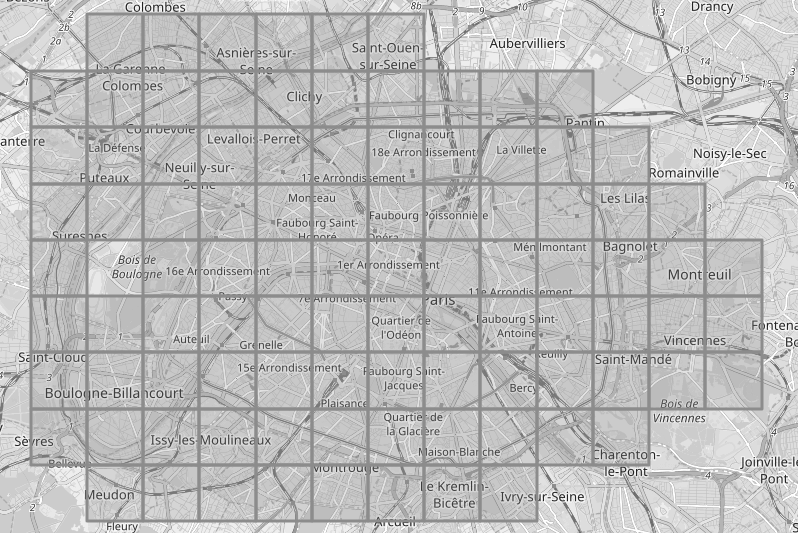
\includegraphics[width=.8\linewidth]{static/gridification_for_paris_gray.png}
\end{center}

After gridification, the ad-hoc orders within a pixel are aggregated by their
    placement timestamps into sub-daily time steps of pre-defined lengths
    to obtain a time table as exemplified in Figure \ref{f:timetable} with
    one-hour intervals.

\begin{center}
\captionof{figure}{Aggregation into a time table with hourly time steps}
\label{f:timetable}
\begin{tabular}{|c||*{9}{c|}}
    \hline
    \backslashbox{Time}{Day} & \makebox[2em]{\ldots}
        & \makebox[3em]{Mon} & \makebox[3em]{Tue}
        & \makebox[3em]{Wed} & \makebox[3em]{Thu}
        & \makebox[3em]{Fri} & \makebox[3em]{Sat}
        & \makebox[3em]{Sun} & \makebox[2em]{\ldots} \\
    \hline
    \hline
    11:00 & \ldots & $y_{11,Mon}$ & $y_{11,Tue}$ & $y_{11,Wed}$ & $y_{11,Thu}$
                   & $y_{11,Fri}$ & $y_{11,Sat}$ & $y_{11,Sun}$ & \ldots \\
    \hline
    12:00 & \ldots & $y_{12,Mon}$ & $y_{12,Tue}$ & $y_{12,Wed}$ & $y_{12,Thu}$
                   & $y_{12,Fri}$ & $y_{12,Sat}$ & $y_{12,Sun}$ & \ldots \\
    \hline
    \ldots & \ldots & \ldots & \ldots & \ldots
           & \ldots & \ldots & \ldots & \ldots & \ldots \\
    \hline
    20:00 & \ldots & $y_{20,Mon}$ & $y_{20,Tue}$ & $y_{20,Wed}$ & $y_{20,Thu}$
                   & $y_{20,Fri}$ & $y_{20,Sat}$ & $y_{20,Sun}$ & \ldots \\
    \hline
    21:00 & \ldots & $y_{21,Mon}$ & $y_{21,Tue}$ & $y_{21,Wed}$ & $y_{21,Thu}$
                   & $y_{21,Fri}$ & $y_{21,Sat}$ & $y_{21,Sun}$ & \ldots \\
    \hline
    \ldots & \ldots & \ldots & \ldots & \ldots
           & \ldots & \ldots & \ldots & \ldots & \ldots \\
    \hline
\end{tabular}
\end{center}
\

Consequently, each $y_{t,d}$ in Figure \ref{f:timetable} is the number of
    all orders within the pixel for the time of day $t$ and day of week
    $d$ ($y_t$ and $y_{t,d}$ are the same but differ in that the latter
    acknowledges a 2D view).
The same trade-off as with gridification applies:
The shorter the interval, the weaker is the demand pattern to be expected in
    the time series due to less aggregation while longer intervals lead to
    less usable forecasts.
We refer to time steps by their start time, and their number per day, $H$,
    is constant.
Given a time table as in Figure \ref{f:timetable} there are two ways to
    generate a time series by slicing:
\begin{enumerate}
    \item \textbf{Horizontal View}:
    Take only the order counts for a given time of the day
    \item \textbf{Vertical View}:
    Take all order counts and remove the double-seasonal pattern induced
    by the weekday and time of the day with decomposition
\end{enumerate}
Distinct time series are retrieved by iterating through the time tables either
    horizontally or vertically in increments of a single time step.
Another property of a generated time series is its length, which, following
    the next sub-section, can be interpreted as the sum of the production
    training set and the test day.
In summary, a distinct time series is generated from the tabular order data
    based on a configuration of parameters for the dimensions pixel size,
    number of daily time steps $H$, shape (horizontal vs. vertical), length,
    and the time step to be predicted.
